\documentclass[border=8pt]{standalone}
\usepackage{amsmath}
\usepackage{tikz}
\usetikzlibrary{arrows.meta,decorations.pathmorphing}
\definecolor{navy}{HTML}{1A1D21}
\definecolor{blue}{HTML}{0D9488}
\definecolor{softblue}{HTML}{CFEDEA}
\definecolor{paper}{HTML}{EEF0F3}
\definecolor{muted}{HTML}{646A72}
\definecolor{orange}{HTML}{E05A47}
\begin{document}
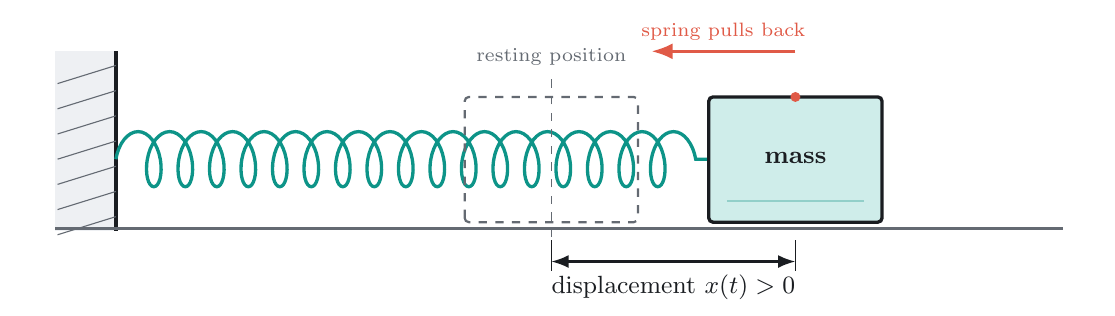
\begin{tikzpicture}[x=1cm,y=1cm,>=Latex]
  \path[use as bounding box] (-0.2,-0.75) rectangle (13.25,2.55);

  % Wall and smooth supporting surface.
  \fill[paper] (0.15,-0.03) rectangle (0.92,2.25);
  \draw[navy,very thick] (0.92,-0.03)--(0.92,2.25);
  \foreach \y in {0.10,0.42,...,2.18}{
    \draw[muted,thin] (0.18,\y-0.18)--(0.92,\y+0.05);
  }
  \draw[muted,thick] (0.15,0)--(12.95,0);

  % The spring is stretched from the wall to the displaced mass.
  \draw[blue,very thick,decorate,
    decoration={coil,aspect=0.52,segment length=4.0mm,amplitude=3.5mm}]
    (0.92,0.88)--(8.45,0.88);

  % A faint equilibrium position makes the displacement visible.
  \draw[muted,dashed,thick,rounded corners=1.5pt]
    (5.35,0.08) rectangle (7.55,1.67);
  \draw[muted,dashed] (6.45,-0.11)--(6.45,1.93);
  \node[font=\scriptsize,color=muted,anchor=south] at (6.45,1.95)
    {resting position};

  % The released mass and the spring's restoring force.
  \draw[navy,very thick,fill=softblue,rounded corners=1.5pt]
    (8.45,0.08) rectangle (10.65,1.67);
  \draw[blue!45,line width=0.55pt]
    (8.68,0.35)--(10.42,0.35);
  \node[font=\bfseries\small,color=navy] at (9.55,0.90) {mass};
  \fill[orange] (9.55,1.67) circle (1.8pt);
  \draw[orange,very thick,-{Latex[length=2.7mm]}]
    (9.55,2.25)--(7.72,2.25)
    node[midway,above,font=\scriptsize] {spring pulls back};

  % Displacement measured from equilibrium.
  \draw[navy,thin] (6.45,-0.15)--(6.45,-0.54);
  \draw[navy,thin] (9.55,-0.15)--(9.55,-0.54);
  \draw[navy,thick,{Latex[length=2.2mm]}-{Latex[length=2.2mm]}]
    (6.45,-0.42)--(9.55,-0.42)
    node[midway,below=1pt,font=\small] {displacement $x(t)>0$};
\end{tikzpicture}
\end{document}
